\documentclass{article}
% chktex-file 44
% chktex-file 8
% chktex-file 18
% chktex-file 35
\usepackage[margin=1in]{geometry}
\usepackage{amsmath}
\usepackage{amssymb}
\usepackage{bm}
\usepackage{pdfpages}
\usepackage{graphicx}
\usepackage{mathtools}
\usepackage{eurosym}
\usepackage[hidelinks]{hyperref}
\usepackage{float}

\usepackage{fancyhdr}
\pagestyle{fancy}
\lhead{Ahou L. -  Ahou S. - Fiorini L. - Portier A.} % controls the left corner of the header
\chead{} % controls the center of the header
\rhead{Groupe 49} % controls the right corner of the header
\lfoot{} % controls the left corner of the footer
\cfoot{} % controls the center of the footer
\cfoot{~\thepage} % controls the right corner of the footer
\usepackage{titlesec}

% Commands for physic unit
\newcommand{\unit}[1]{[\mathrm{#1}]}

\begin{document}

\section*{Question 4A}
Puisque nous nous intéressons seulement aux bilans de productions/consommations et du niveau du bassin
sur des périodes de $T \unit{h}$, nous pouvons exprimer toutes nos variables en fonction de cette période.\\
Voici deux tableaux reprenant les notations principales utilisées dans cette seconde partie \footnote{Toutes autres notations utilisées dans la suite seront définies lorsque celles-ci seront introduites} : 

\begin{table}[h!]
    \centering
    \renewcommand{\arraystretch}{1.5}% Add spacing between rows : default value is 1
    \begin{tabular}{|c || c |} 
        \hline
        Nom & Signification\\
        \hline\hline
        $c_i$ & Capacité éolienne installée sur le i\textsuperscript{ème} site\\
        $t_j$ & Puissance à envoyer en turbinage choisie durant la j\textsuperscript{ème} période\\
        $p_j$ & Puissance de pompage choisie durant la j\textsuperscript{ème} période\\
        \hline
    \end{tabular}
    \caption{Table des notations des variables de décisions utilisées pour le modèle de la question 4.}
    \label{table:notations_variables_4}
\end{table}

\begin{table}[h!]
    \centering
    \renewcommand{\arraystretch}{1.5}% Add spacing between rows : default value is 1
    \begin{tabular}{|c || p{14cm} |} 
        \hline
        Nom & Signification\\
        \hline\hline
        $n$ & Nombre de sites éoliens \\
        $m$ & Nombre de périodes de $T \unit{h}$ dans une année\\
        $e_i(j)$ & Rendement éolien du i\textsuperscript{ème} site durant la j\textsuperscript{ème} période\\
        $a_j$ & Apport fluvial durant la j\textsuperscript{ème} période\\
        $\mathrm{cons}_j$ & Consommation énergétique durant la j\textsuperscript{ème} période\\
        $t_\mathrm{max}$ & Capacité maximale d'énergie générée par le turbinage (Sur une période de T heures)\\
        $p_\mathrm{max}$ & Capacité maximale de pompage (Sur une période de T heures)\\
        $\mathrm{stock}_\mathrm{max}$ & Capacité de stockage maximale\\
        $\eta$ & Rendement de turbinage\\
        $\mathrm{costs}$ & Vecteur donnant les valeurs du coût d'installation d'un site éolien  (onshore/offshore) \newline $\mathrm{costs}_i = $ Coût d'installation d'un site onshore si le site d'index $i$ est onshore, et inversement.\\  
        \hline
    \end{tabular}
    \caption{Table des notations des constantes utilisées pour le modèle.}
    \label{table:notations_constantes}
\end{table}

\noindent
Le modèle peut alors s'écrire ainsi :
\begin{align}
    \min_{c_{i},t_j,p_j} \quad &\mathrm{costs}^\intercal\mathbf{c} \nonumber\\
    \textrm{tel que} \quad & \sum_{i=0}^{n-1} c_i e_i(j) + \eta \cdot t_j - p_j \ge \mathrm{cons}_j \quad \forall j \in  \{ 0, \ldots, m-1 \}\label{eq:4A_contr1}\\
    & 0 \le \frac{\mathrm{stock}_\mathrm{max}}{2}  + \sum_{j=0}^{k} p_j - t_j + a_j \le  \mathrm{stock}_\mathrm{max} \quad \forall k \in \{ 0, \ldots, m-2 \}\label{eq:4A_contr2}\\
    & \sum_{j=0}^{m-1} p_j - t_j + a_j = 0 \label{eq:4A_contr3}\\
    & 0 \le c_i \le c_i^\mathrm{max} \quad \forall i \in  \{ 0, \ldots, n-1 \}  \label{eq:4A_contr4}\\
    & 0 \le \eta \cdot t_j \le  t_\mathrm{max} \quad \forall j \in  \{ 0, \ldots, m-1 \}  \label{eq:4A_contr5}\\
    & 0 \le p_j \le  p_\mathrm{max} \quad \forall j \in  \{ 0, \ldots, m-1 \} \label{eq:4A_contr6}
\end{align}

\newpage

La fonction objectif représente le coût total d'installation des éoliennes (en tenant compte des différences entre les installations \textit{offshore} et \textit{onshore}). \\
La contrainte \eqref{eq:4A_contr2} fait le bilan lié aux variations des opérations de turbinage/pompage décidées et de l'apport fluvial naturel depuis le temps $t = 0$ jusqu'en tout temps $t = k$ afin de calculer l'augmentation/la diminution du niveau de l'eau dans le bassin.\\
La formalisation peut s'obtenir en sachant que le niveau initial de notre bassin est à $0.5 \times \mathrm{stock}_\mathrm{max}$, puis que le niveau du bassin au prochain temps est le niveau du bassin passé plus les fluctuations à la période $j$, pompage - turbinage + apport fluvial, qui est donné plus formellement par $\mathrm{bassin}_{j+1} = \mathrm{bassin}_{j} + p_j - t_j + a_j$, donc en développant cette relation de récurrence, nous obtenons 
bien le niveau de notre bassin pour toute période $j \in \{ 0, \ldots, m-1 \}$ en fonction de nos variables, et en sachant que le niveau du bassin doit revenir à son niveau initial, à la fin 
de la période considérée, il y a une contrainte "en moins" pour \eqref{eq:4A_contr2} qui apparaît dans \eqref{eq:4A_contr3}. \\
La contrainte \eqref{eq:4A_contr3} indique que le niveau final du bassin doit revenir au même niveau qu'initialement. Autrement dit, les opérations de turbinage/pompage et 
l'apport fluvial doivent se sommer à 0 à la fin de la dernière période.\\
Les contraintes \eqref{eq:4A_contr4}, \eqref{eq:4A_contr5} et \eqref{eq:4A_contr6} indiquent respectivement les bornes sur les capacités éoliennes maximales installables sur chaque site, 
les capacités maximales de turbinages et les capacités maximales de pompages pour des périodes de $T \unit{h}$, regroupées au niveau européen, bien entendu.
Nous avons cependant supposé pour la \eqref{eq:4A_contr5} contrainte, liée au turbinage, que la valeur $t_j$ est ce que 
nous extrayons du bassin, puis
la capacité $t_\mathrm{max}$ restreint alors l'énergie en sorte de la turbine($\eta \cdot t_j$), qui sert à la 
production électrique dans la condition \eqref{eq:4A_contr1}.

\newpage % Car il faudra rendre sur Gradescope en séparant les questions

\section*{Question 4B}
Suite à l'implémentation de notre problème d'optimisation sur le notebook Jupyter, nous obtenons 
un coût moyen qui est d'environ $\mathbf{58.282}$\euro/MWh. \footnote{C'est une valeur qui semble cohérente, surtout pour un modèle comme ici, 
assez libre et qui ne prétend pas refléter les réalités, le prix moyen de l'énergie par MWh en Europe actuellement 
est aux alentours de quelques centaines d'euros, d'après la Commission européenne : 
\url{https://ec.europa.eu/eurostat/statistics-explained/index.php?title=Electricity_price_statistics}, 
consulté le 8 mai 2024 à 01h08.} Nous avons implémenté ce problème avec la bibliothèque CVXPY qui a été recommandée, cependant
il y a plusieurs solvers disponibles et ils donnent pour ceux qui ont été testé, des résultats différents (pour le choix des valeurs de décision) mais qui arrivent presque à
la même valeur de fonction objectif, la différence étant sûrement due aux erreurs de calcul numérique. Pour cette résolution,
nous avons utilisé "SCIPY" (la liste des solvers étant disponible ici : \url{https://www.cvxpy.org/tutorial/solvers/index.html}), c'est le solver
avec lequel nous avons eu le plus de performance, en terme de rapidité de calcul, et il semblait plus cohérent et consistant que les autres
sur les résultats, donc nous en avons fait le choix.


\begin{figure}[h!]
    \centering
    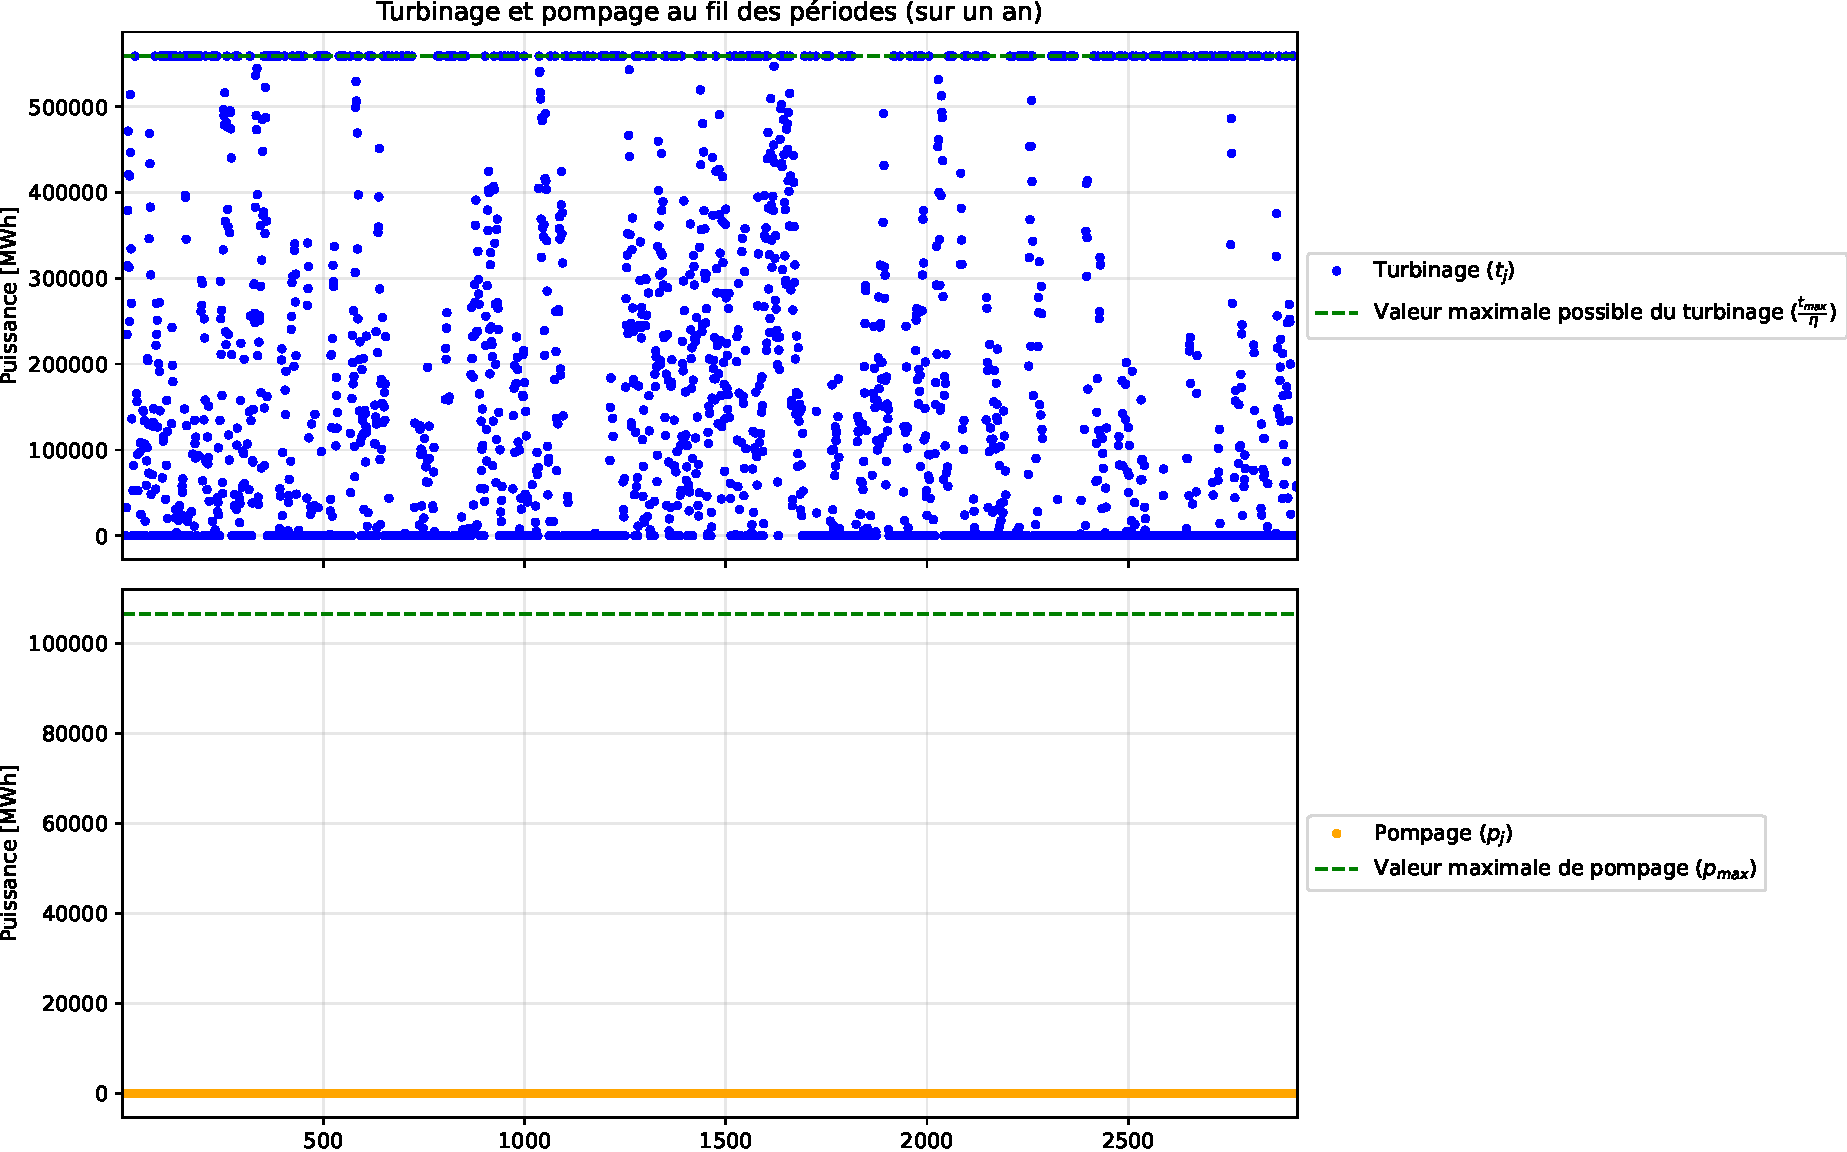
\includegraphics[scale=0.6]{GraphesP2/Turbinage_pompage_Q4.pdf}
    \caption{Représentation graphique du turbinage et du pompage
    influençant le niveau du bassin \eqref{eq:4A_contr2} pour le modèle de la question 4 par période de T = 3 heures sur un an.}
    \label{fig:Turbinage_pompage_Q4}
\end{figure}
\newpage
\begin{figure}[h!]
    \centering
    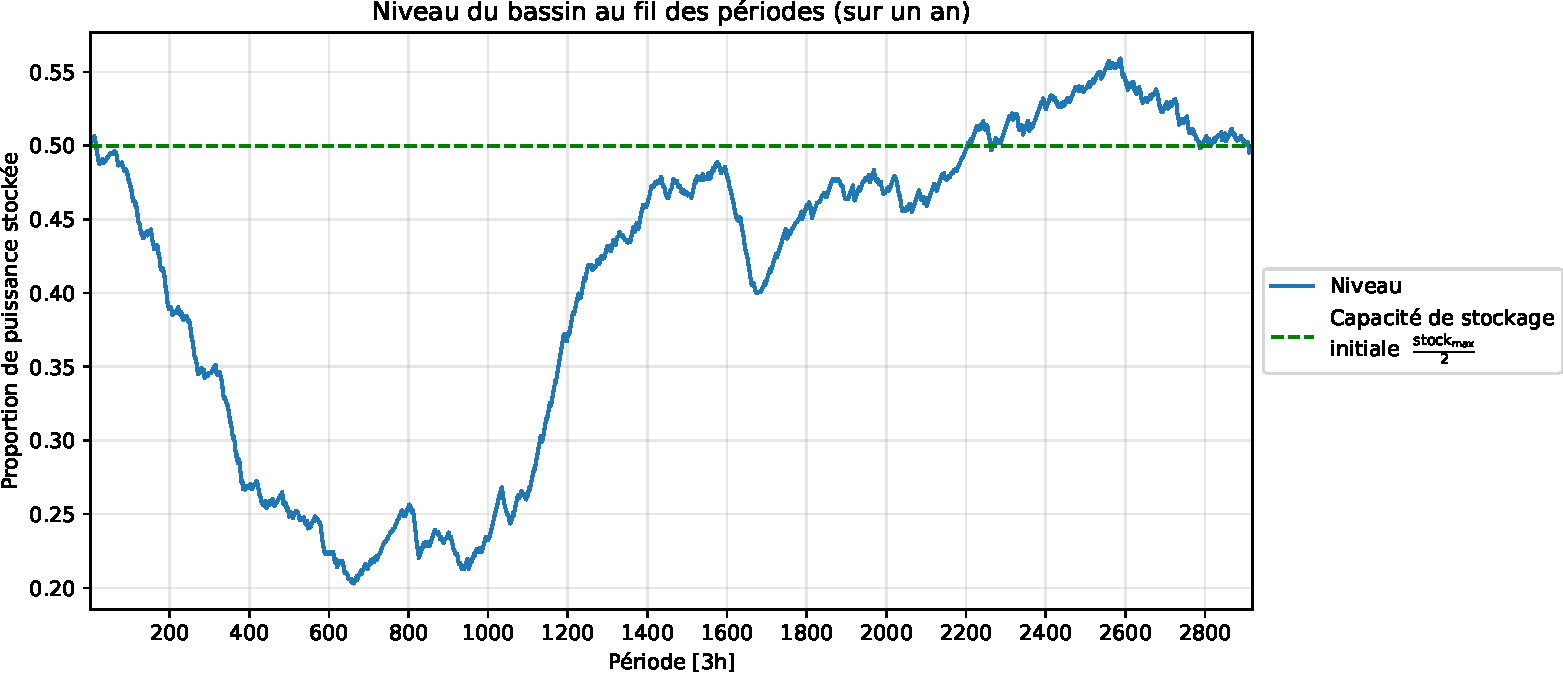
\includegraphics[scale=0.6]{GraphesP2/Niveau_Bassin_Q4.pdf}
    \caption{Représentation graphique du niveau du bassin \eqref{eq:4A_contr2} pour le modèle 
    de la question 4 par période de T = 3 heures sur un an.}
    \label{fig:Niveau_bassin_Q4}
\end{figure}
\noindent Le graphique indique bien que nous remontons au niveau initial à la fin de l'année. \\

\begin{figure}[h!]
    \centering
    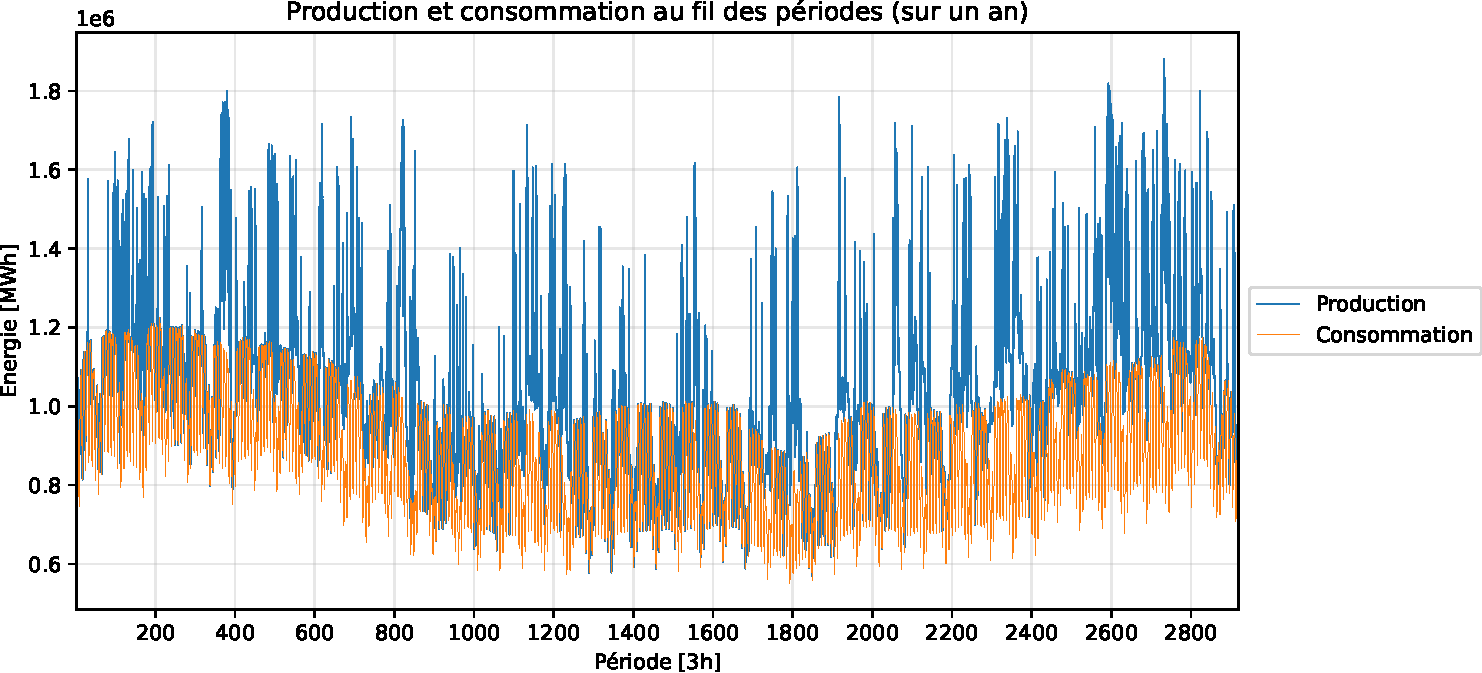
\includegraphics[scale=0.6]{GraphesP2/Prod_Cons_Q4.pdf}
    \caption{Représentation graphique de la production et de la consommation (en MWh) \eqref{eq:4A_contr1} pour le modèle de la question 4 
    par période de T = 3 heures sur un an.}
    \label{fig:Prod_Cons_Q4}
\end{figure}

\noindent Nous pouvons voir quelques écarts significatifs entre la production et la consommation, c'est-à-dire 
qu'à certains moments, nous "gaspillons" de l'énergie car nous produisons trop (où nous avons bien retiré à la production l'énergie stockée dans le bassin, donc il s'agit d'une perte sèche).


\clearpage
\section*{Question 4C}
Pour traiter cette question, il faut s'intéresser au problème dual, une formulation pratique est la forme standard, qui nous 
permet d'exploiter les aspects théoriques de la méthode du simplexe afin de voir l'influence d'une quantité sur le coût total.
En réajustant le modèle dans la bonne formulation, nous avons alors 
\begin{align}
    \min_{c_{i},t_j,p_j} \quad &\mathrm{costs}^\intercal\mathbf{c} \nonumber\\
    \textrm{tel que} \quad  \sum_{i=0}^{n-1} c_i e_i(j) + \eta \cdot t_j - p_j &\ge \mathrm{cons}_j \quad \forall j \in  \{ 0, \ldots, m-1 \}\label{eq:4C_contr1}\\
     \sum_{j=0}^{k} p_j - t_j + a_j &\ge  -\frac{\mathrm{stock}_\mathrm{max}}{2} \quad \forall k \in \{ 0, \ldots, m-2 \}\label{eq:4C_contr20}\\
    -\sum_{j=0}^{k} p_j - t_j + a_j &\ge  -\frac{\mathrm{stock}_\mathrm{max}}{2} \quad \forall k \in \{ 0, \ldots, m-2 \}\label{eq:4C_contr21}\\
     \sum_{j=0}^{m-1} p_j - t_j + a_j &= 0 \label{eq:4C_contr3}\\
     -c_i &\ge -c_i^\mathrm{max}  \quad \forall i \in  \{ 0, \ldots, n-1 \}  \label{eq:4C_contr40}\\
    - \eta \cdot t_j &\ge  -t_\mathrm{max} \quad \forall j \in  \{ 0, \ldots, m-1 \}  \label{eq:4C_contr50}\\
     -p_j &\ge  -p_\mathrm{max} \quad \forall j \in  \{ 0, \ldots, m-1 \} \label{eq:4C_contr60}\\
     c_i &\ge 0  \quad \forall i \in  \{ 0, \ldots, n-1 \}   \label{eq:4C_contr41}\\
     t_j &\ge  0 \quad \forall j \in  \{ 0, \ldots, m-1 \}  \label{eq:4C_contr51}\\
     p_j &\ge  0 \quad \forall j \in  \{ 0, \ldots, m-1 \} \label{eq:4C_contr61}
\end{align}
Sous cette forme, nous pouvons reconnaître une formulation de type $Ax \geq b, x \geq 0$ (sauf pour l'égalité, 
mais ça peut facilement se lire comme deux inégalités, et vu que $\eta > 0$, $\eta \cdot t_j \geq 0 \iff t_j \geq 0$). Dès lors, en introduisant des variables d'écarts pour chaque inégalité ($-s_i$ et telles que $s_i \geq 0$ pour toute inégalité), nous
pouvons facilement avoir une formulation de type $Ax = b, x \geq 0$, qui nous convient parfaitement pour le simplexe, surtout sachant que les 
variables d'écarts ne vont pas intervenir dans la fonction objectif donc leur valeur n'importera pas pour la question. Bien que ça ne soit 
pas la formulation la plus rigoureuse, il vaut mieux procéder ainsi afin d'éviter des notations trop lourdes, nous arrivons
facilement à identifier dans la méthode du simplexe, puisque nous avons une solution optimale bien finie, qu'il existe deux sous-matrices
$B$ et $N$ de notre matrice $A$ reprenant les éléments à gauche de notre formulation, que nous avons un vecteur 
$b$ qui reprend les éléments
$(\mathrm{cons}_0, \ldots, \mathrm{cons}_{m-1}, -\frac{\mathrm{stock}_\mathrm{max}}{2}, \ldots, 
-\frac{\mathrm{stock}_\mathrm{max}}{2}, -\frac{\mathrm{stock}_\mathrm{max}}{2}, \ldots, 
-\frac{\mathrm{stock}_\mathrm{max}}{2},$ \\ $ 0, -c_0^\mathrm{max}, \ldots, -c_{n-1}^\mathrm{max},
-t_\mathrm{max}, \ldots, -t_\mathrm{max}, -p_\mathrm{max}, \ldots, -p_\mathrm{max}) $. \\ 
Nous avons aussi le vecteur des coûts, qui peut se décomposer en coûts concernant les éléments de la base, et les éléments nuls,
bien évidemment, ça ne change rien de réorganiser le tout au niveau des variables, 
$\mathrm{costs}^\intercal = (\mathrm{costs}^\intercal_{B}, \mathrm{costs}^\intercal_{N})$.
Selon la théorie, notre coût optimal est donné par $\mathrm{costs}^\intercal_{B} B^{-1} b$.


\subsection*{Stockage}
Si nous augmentons d'une unité notre stockage, nous avons donc que $\mathrm{stock}_\mathrm{max} \leftarrow \mathrm{stock}_\mathrm{max} + 1$ (réassignation), donc dans notre modèle,
notre vecteur $b$ est modifié, et devient $b$ plus un vecteur comprenant $- \frac{1}{2}$ pour les contraintes 
$\eqref{eq:4C_contr20}$ et $\eqref{eq:4C_contr21}$ et 0 sinon. Notons $\mathbf{1}_{\mathrm{stock}}$ le vecteur ayant pour composante $1$ si 
la contrainte associée est dans $\eqref{eq:4C_contr20}$ ou $\eqref{eq:4C_contr21}$, et ayant une composante nulle sinon. Rajouter une unité de stockage 
revient à dire que $b \leftarrow b  - \frac{1}{2} \mathbf{1}_{\mathrm{stock}}$, 
dès lors notre coût optimal devient $\mathrm{costs}^\intercal_{B} B^{-1} \left( b - \frac{1}{2} \mathbf{1}_{\mathrm{stock}} \right) 
= \mathrm{costs}^\intercal_{B} B^{-1} b - \frac{1}{2} \mathrm{costs}^\intercal_{B} B^{-1} \mathbf{1}_{\mathrm{stock}}  $ où le premier terme
est connu puisque c'est la valeur de notre coût total, et la second partie peut être calculée, car $\mathrm{costs}^\intercal_{B} B^{-1}$ correspond
à la transposée du vecteur de solution optimale du problème dual, qui peut facilement être obtenu par CVXPY. Sur le notebook Jupyter, nous calculons 
que cela ne change pas le coût optimal, donc \underline{l'augmentation de notre capacité de stockage d'une unité ne rapporte pas d'argent}.

\subsection*{Pompage}
Procédons de la même manière que pour le stockage, nous voulons augmenter la capacité de pompage d'une unité, pour cela, étant donné que
notre modèle se base sur des périodes de 3 heures, nous devons multiplier par 3 notre augmentation, donc cela nous donne $p_\mathrm{max} \leftarrow p_\mathrm{max} + 3$,
et pour le vecteur $b$, il faut regarder aux contraintes \eqref{eq:4C_contr60}, en définissant de la même manière $\mathbf{1}_{\mathrm{p}}$, qui est composé
de $1$ si la contrainte associée à la composante est dans $\eqref{eq:4C_contr60}$ et $0$ sinon. Notre coût optimal nous sera donné par 
$\mathrm{costs}^\intercal_{B} B^{-1} \left( b - 3 \cdot \mathbf{1}_{p} \right) 
= \mathrm{costs}^\intercal_{B} B^{-1} b - 3 \cdot \mathrm{costs}^\intercal_{B} B^{-1} \mathbf{1}_{p}  $.
Après l'implémentation sur Python, nous avons aussi que le coût optimal reste le même, donc \underline{l'augmentation de notre capacité de pompage d'une unité 
ne rapporte pas d'argent}

\subsection*{Turbinage}
Nous pouvons aussi faire les choses de la même façon, il faut réassigner notre valeur de turbinage en lui ajoutant 3 car nous travaillons
sur des périodes de 3 heures, donc $t_\mathrm{max} \leftarrow t_\mathrm{max} + 3$, ensuite nous devons définir le vecteur $\mathbf{1}_{t}$ qui comme avant 
a pour valeur 1 si sa contrainte associée est dans \eqref{eq:4C_contr50}, 0 sinon. Notre coût optimal nous sera donné par 
$\mathrm{costs}^\intercal_{B} B^{-1} \left( b - 3 \cdot \mathbf{1}_{t} \right) 
= \mathrm{costs}^\intercal_{B} B^{-1} b - 3 \cdot \mathrm{costs}^\intercal_{B} B^{-1} \mathbf{1}_{t}  $. D'après notre code, nous trouvons une diminution
de notre coût de $\mathbf{1.583.760,79}$\euro, ce qui est sûrement dû au fait que notre capacité de turbinage supplémentaire nous permet de mieux
exploiter l'afflux naturel d'eau et de gaspiller moins d'énergie en surproduisant au-dessus de la demande. \\

\noindent \textit{Tout notre raisonnement reste valide par rapport aux contraintes car nous considérons que pour des petites variations, notre solution reste admissible.}

\newpage
\section*{Question 5}
Nous devons à présent choisir, pour chaque site d'éoliennes, si nous installons $0\%, 50\%$ ou $100\%$ de la capacité maximale installable sur ce site.
Pour ce faire, nous rédéfinissons les variables $c_i$ de la question 4 :

\begin{table}[h!]
    \centering
    \renewcommand{\arraystretch}{1.5}% Add spacing between rows : default value is 1
    \begin{tabular}{|c || c |} 
        \hline
        Nom & Signification\\
        \hline\hline
        $c_{i} \in \{ 0, 1, 2 \}$ & Proportion de la capacité maximale $c_i^\mathrm{max}$ installée sur le i\textsuperscript{ème} site\\
        $t_j$ & Puissance à envoyer en turbinage choisie durant la j\textsuperscript{ème} période\\
        $p_j$ & Puissance de pompage choisie durant la j\textsuperscript{ème} période\\
        \hline
    \end{tabular}
    \caption{Table des nouvelles notations des variables de décisions utilisées pour le modèle de la question 5.}
    \label{table:notations_variables_5}
\end{table} 

\noindent La puissance installée sur le i\textsuperscript{ème} site équivaut alors à $0.5 \cdot c_ic_i^\mathrm{max}$. Le modèle devient alors :
\begin{align}
    \min_{c_{i} \in \mathbb{Z},t_j,p_j} \quad &\mathrm{costs}^\intercal 
    \begin{pmatrix}
        0.5 \cdot c_0c_0^\mathrm{max}\\
        \vdots\\
        0.5 \cdot c_{n-1}c_{n-1}^\mathrm{max}
    \end{pmatrix} \nonumber\\
    \textrm{tel que} \quad & \sum_{i=0}^{n-1} 0.5 \cdot c_ic_i^{max} e_i(j) + \eta \cdot t_j - p_j \ge \mathrm{cons}_j \quad \forall j \in  \{ 0, \ldots, m-1 \}\label{eq:5_contr1}\\
    & 0 \le \frac{\mathrm{stock}_\mathrm{max}}{2}  + \sum_{j=0}^{k} p_j - t_j + a_j \le  \mathrm{stock}_\mathrm{max} \quad \forall k \in \{ 0, \ldots, m-2 \}\label{eq:5_contr2}\\
    & \sum_{j=0}^{m-1} p_j - t_j + a_j = 0 \label{eq:5_contr3}\\
    & 0\le c_i \le 2 \quad \forall i \in  \{ 0, \ldots, n-1 \} \label{eq:5_contr4}  \\
    & 0 \le \eta \cdot t_j \le  t_\mathrm{max} \quad \forall j \in  \{ 0, \ldots, m-1 \} \label{eq:5_contr5}\\
    & 0 \le p_j \le  p_\mathrm{max} \quad \forall j \in  \{ 0, \ldots, m-1 \} \label{eq:5_contr6} 
\end{align}
Ici, nous avons gardé les mêmes contraintes sauf pour celles concernant les $c_i$, la \eqref{eq:5_contr4} nous dit bien
que les $c_i$ sont entre 0 et 2, et vu qu'ils sont entiers, nous avons bien nos valeurs atetndues, ensuite la \eqref{eq:5_contr1}
nous donne la même contrainte par rapport au fait que la consommation doit être satisfaite, sauf qu'il faut ajuster
les $c_i$ pour qu'ils nous donnent 0, 50\% et 100\% de la capacité maximale. Il y a également eu un léger changement dans la 
fonction objectif. \\
Pour la résolution de ce modèle, nous avons dû réduire la durée étudiée, en effet, nous avons tout d'abord
testé avec 2920 périodes (au complet), avec le solver par défaut de CVXPY, nous avions dépassé les 180 minutes
d'exécution et avons alors arrêté, ensuite nous avons testé avec le solver SCIPY et avons arrêté au-dessus de 120
minutes, nous avons en premier lieu ensuite réduit le nombre de périodes à 1500, nous avions excédé les 65
minutes avec encore le solver SCIPY. Enfin, nous avons défini le nombre de périodes à \textbf{1000}, et nous arrivons
à \textbf{46 minutes et 10.5 secondes} de calcul, donc nous avons conclu que notre choix de durée était raisonnable.
Lorsque nous résolvons notre modèle avec SCIPY pour 1000 périodes, nous obtenons un coût total de "$125.935.889.457,89$ \euro", mais il reste
à déterminer quelle est la bonne unité, en sachant que nos $c_i^{max}$ sont en $MW$, si nos coûts d'installations peuvent être amortis sur une sous-période, chose très improbable, nous aurions
alors des $\frac{\text{\euro}}{MW \cdot 1000 p}$ (en notant 1000 p le fait que nous avons 1000 périodes et en sachant 
qu'un an = 2920 p)
ce qui nous ferait un coût moyen, en divisant par la consommation sur ces 1000 périodes 
de $131.15 \frac{\text{\euro}}{MWh}$, mais ça ne semble pas être la bonne piste, gardons l'idée de l'amortissement par an, 
nous avons alors un coût total de $125.935.889.457,89 \frac{\text{\euro}}{an}$, si nous divisons par la consommation 
nous avons alors un coût moyen de $131.15 \frac{\text{\euro}}{an}*\frac{1000 p}{ MW}$, 
et si nous souhaitons des $\frac{\text{\euro}}{MWh}$, il suffit 
de multiplier par $an/ 1000 p  = \frac{2920}{1000}$ ce qui nous donne approximativement $\mathbf{382.96} \frac{\text{\euro}}{MWh}$.
Ce coût moyen est bien plus élevé que pour le modèle de la question 4, le temps de calcul a été aussi lourdement impacté, l'optimisation
par la présence des nombres entiers est bien plus complexe, et dans ce cas-ci nous amène un moins bon coût, cela s'explique par le fait qu'il
y a peu de marge sur l'ajustement des sites éoliens, et que le maximum que le solver peut faire c'est d'osciller entre 3 valeurs tout en utilisant
les capacités du bassin le mieux possible.

\begin{figure}[H]
    \centering
    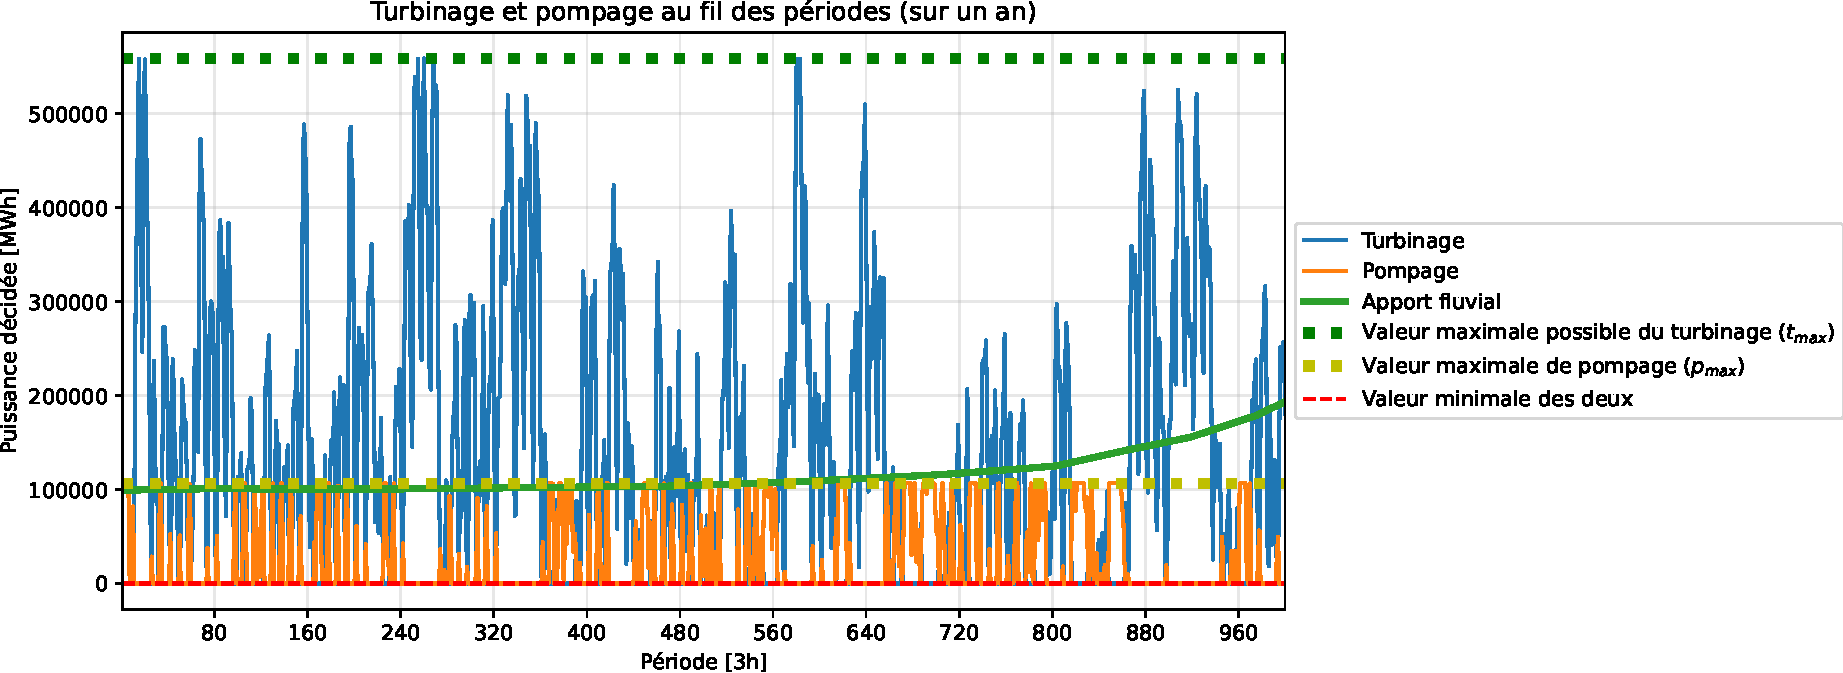
\includegraphics[scale=0.6]{GraphesP2/Turbinage_pompage_Q5.pdf}
    \caption{Représentation graphique du turbinage et du pompage
    influençant le niveau du bassin \eqref{eq:5_contr2} pour le modèle de la question 4 par période de T = 3 heures sur 1000 périodes.}
    \label{fig:Turbinage_pompage_Q5}
\end{figure}

\noindent Dans ce graphique, nous pouvons voir que le turbinage est un peu plus varié qu'à la question 4, moins de valeurs extrêmes (au maximum/minimum), et cette fois-ci,
le pompage est exploité contrairement à la question 4 où il est nul sur toute la période étudiée.

\begin{figure}[H]
    \centering
    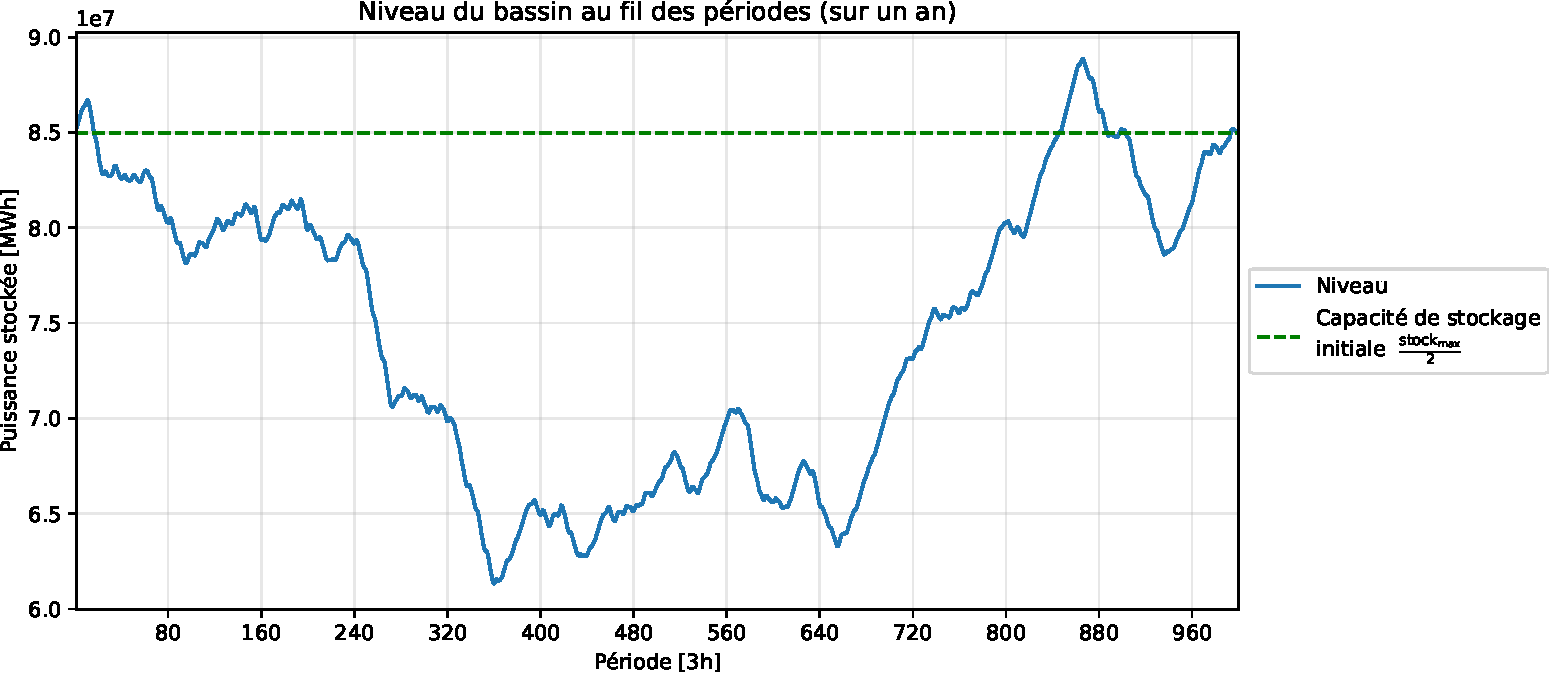
\includegraphics[scale=0.6]{GraphesP2/Niveau_Bassin_Q5.pdf}
    \caption{Représentation graphique du niveau du bassin \eqref{eq:5_contr2} pour le modèle 
    de la question 5 par période de T = 3 heures sur 1000 périodes.}
    \label{fig:Niveau_bassin_Q5}
\end{figure}

\noindent Le graphique indique bien que nous remontons au niveau initial à la fin de la période. 

\begin{figure}[H]
    \centering
    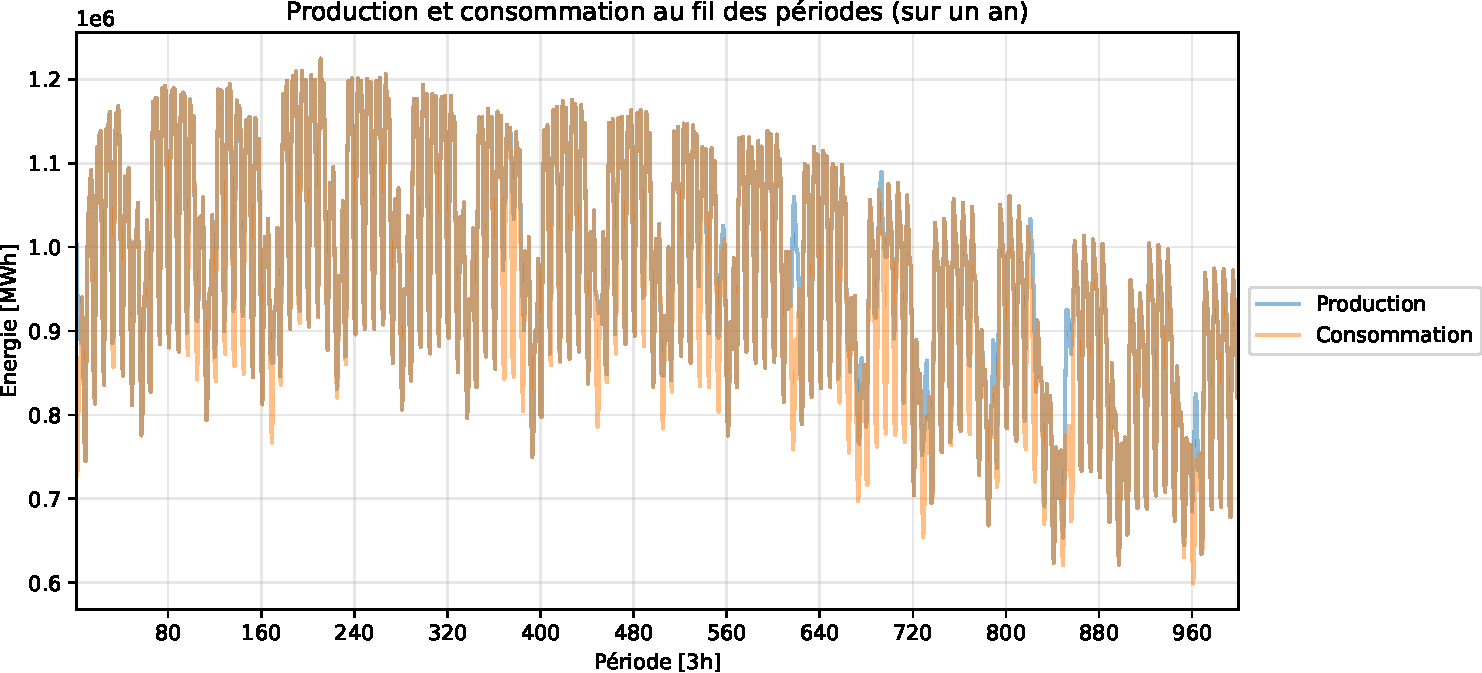
\includegraphics[scale=0.6]{GraphesP2/Prod_Cons_Q5.pdf}
    \caption{Représentation graphique de la production et de la consommation (en MWh) 
    \eqref{eq:5_contr1} pour le modèle de la question 5 par période de T = 3 heures sur 1000 périodes.}
    \label{fig:Prod_Cons_Q5}
\end{figure}
\noindent Nous constatons que la production est beaucoup plus proche de la consommation par rapport à la question précédente.

\clearpage

\section*{Question 6}
Pour ce dernier modèle, nous avons également la possibilité d'installer des centrales à gaz, qui peuvent être utilisées pour produire de l'électricité en cas de besoin.
La puissance totale à installer fait partie des variables de décision, ainsi que l'énergie produite par ces centrales en chaque période de $T \unit{h}$.\\
Nous avons donc les nouvelles variables suivantes :

\begin{table}[h!]
    \centering
    \renewcommand{\arraystretch}{1.5}% Add spacing between rows : default value is 1
    \begin{tabular}{|c || c |} 
        \hline
        Nom & Signification\\
        \hline\hline
        $c_i$ & Capacité éolienne installée sur le i\textsuperscript{ème} site\\
        $t_j$ & Puissance à envoyer en turbinage choisie durant la j\textsuperscript{ème} période\\
        $p_j$ & Puissance de pompage choisie durant la j\textsuperscript{ème} période\\
        $g_\mathrm{tot}$ & Puissance totale à installer pour les centrales à gaz\\
        $g_j$ & \'Energie produite par les centrales à gaz durant la j\textsuperscript{ème} période\\
        \hline
    \end{tabular}
    \caption{Table des notations des variables de décisions utilisées pour le modèle de la question 6.} 
    \label{table:notations_variables_6}
\end{table}

\noindent Nous devons alors prendre en compte, en plus du coût d'installation des éoliennes, le coût d'installation des centrales à gaz ainsi que leur coût de fonctionnement.
Le modèle devient alors :

\begin{align}
    \min_{c_{i},t_j,p_j} \quad &\mathrm{costs}^\intercal\mathbf{c} + \mathrm{gas\_prod\_cost}\cdot \sum_{j=0}^{m-1} g_j + \mathrm{gas\_install\_cost} \cdot g_\mathrm{tot}\nonumber\\
    \textrm{tel que} \quad & \sum_{i=0}^{n-1} c_i e_i(j) + g_j + \eta \cdot t_j - p_j \ge \mathrm{cons}_j \quad \forall j \in  \{ 0, \ldots, m-1 \}\label{eq:6_contr1}\\
    & 0 \le \frac{\mathrm{stock}_\mathrm{max}}{2}  + \sum_{j=0}^{k} p_j - t_j + a_j \le  \mathrm{stock}_\mathrm{max} \quad \forall k \in \{ 0, \ldots, m-2 \}\label{eq:6_contr2}\\
    & \sum_{j=0}^{m-1} p_j - t_j + a_j = 0 \label{eq:6_contr3}\\
    & 0 \le c_i \le c_i^\mathrm{max} \quad \forall i \in  \{ 0, \ldots, n-1 \}  \label{eq:6_contr4}\\
    & 0 \le \eta \cdot t_j \le  t_\mathrm{max} \quad \forall j \in  \{ 0, \ldots, m-1 \}  \label{eq:6_contr5}\\
    & 0 \le p_j \le  p_\mathrm{max} \quad \forall j \in  \{ 0, \ldots, m-1 \} \label{eq:6_contr6}\\
    & 0 \le g_j \le g_\mathrm{tot} \quad \forall j \in  \{ 0, \ldots, m-1 \} \label{eq:6_contr7}
\end{align}

\noindent où $\mathrm{gas\_prod\_cost}$ est le coût de production d'énergie par les centrales à gaz et $\mathrm{gas\_install\_cost}$ est le coût d'installation des centrales à gaz.\\
La fonction objectif tient maintenant compte du coût d'installation et de production des centrales à gaz. La contrainte \eqref{eq:6_contr1} est modifiée pour prendre en compte la production d'énergie par les centrales à gaz dans le bilan total de production. 
Enfin, une dernière contrainte \eqref{eq:6_contr7} est ajoutée pour limiter la production d'énergie par les centrales à gaz à la puissance totale installée.
Après la résolution numérique, nous obtenons une valeur moyenne de $\mathbf{48.15}$ \euro/MWh, ce qui est mieux que 
les résultats de la question 4 ($\mathbf{58.282}$ \euro/MWh) et 5 ($\mathbf{382.96}$ \euro/MWh).
\begin{figure}[H]
    \centering
    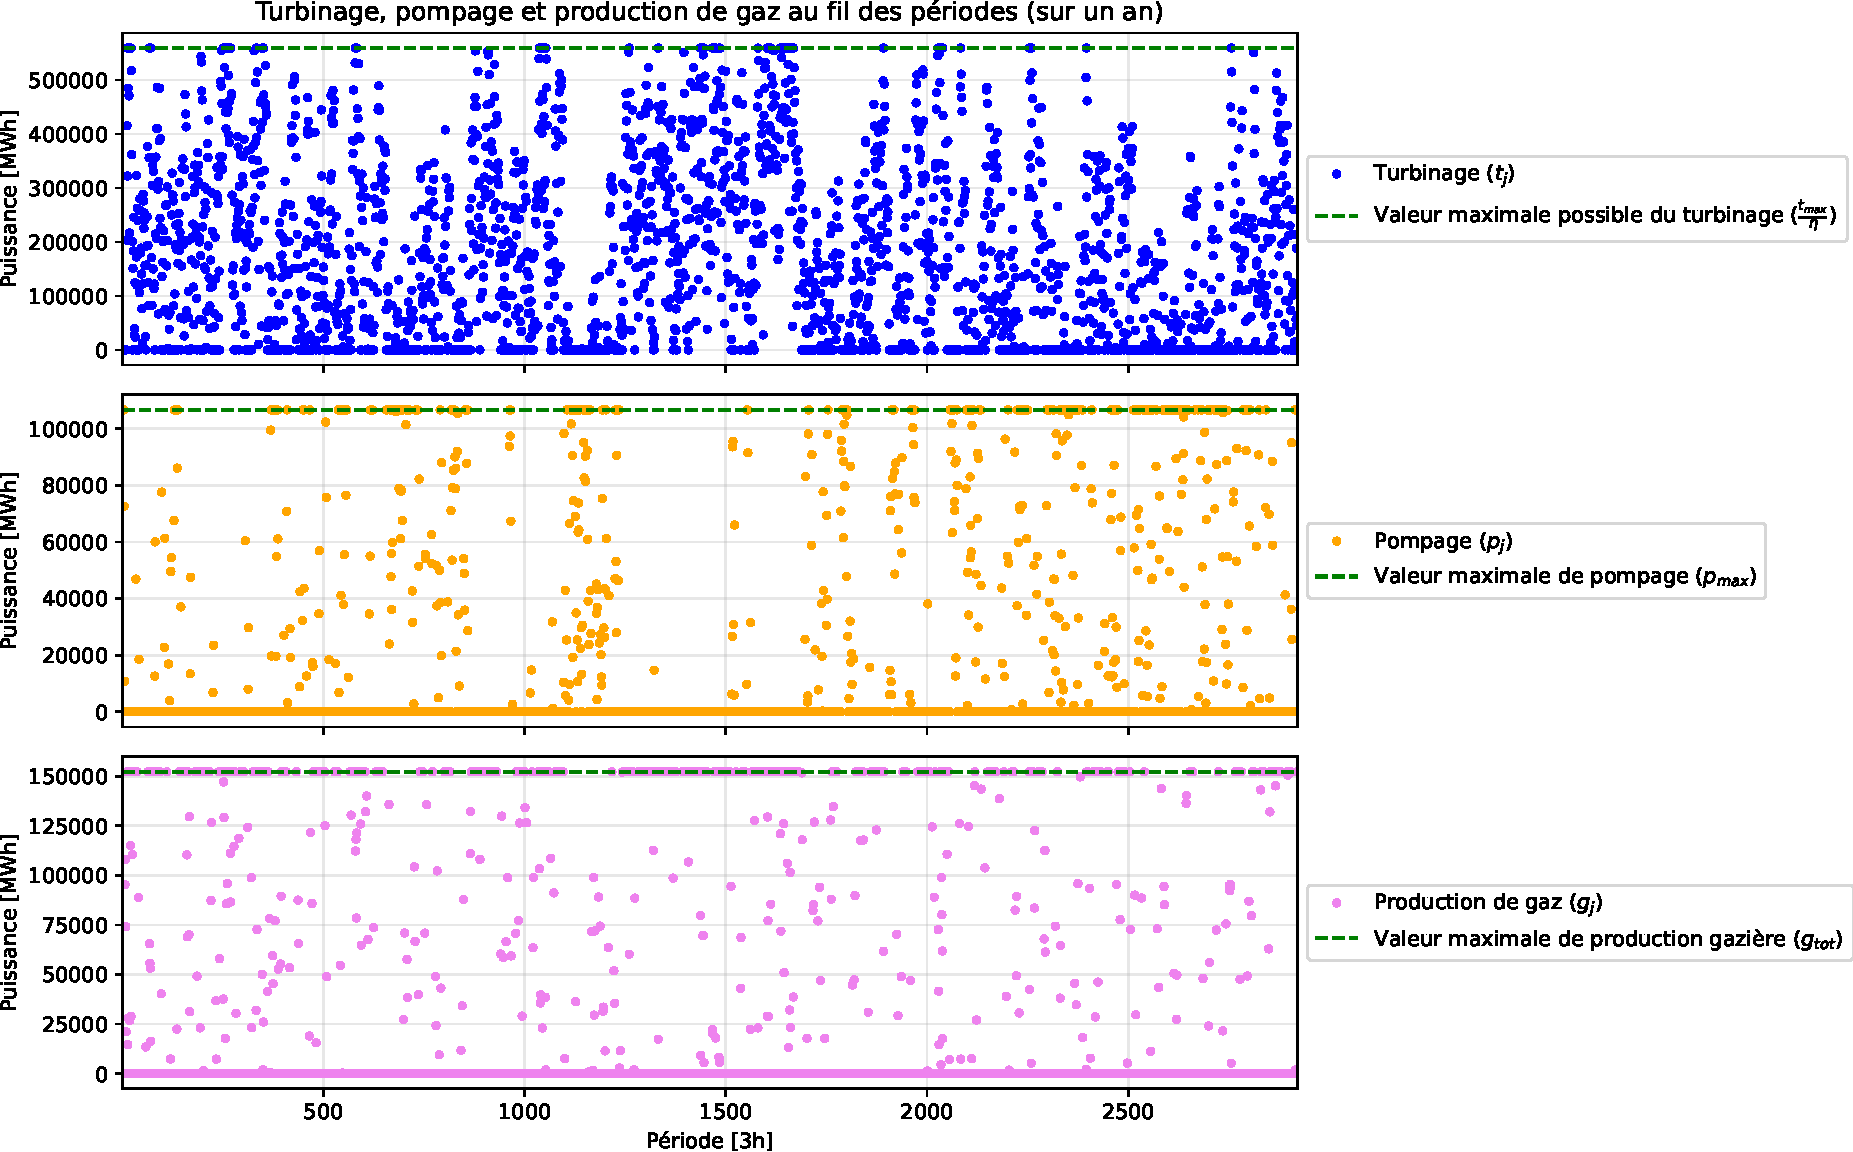
\includegraphics[scale=0.6]{GraphesP2/Productions_Q6.pdf}
    \caption{Représentation graphique du turbinage et du pompage
    influençant le niveau du bassin \eqref{eq:6_contr2} ainsi que de la production de gaz pour le modèle de la question 6 par période de T = 3 heures sur un an.} 
    \eqref{eq:5_contr1}
    \label{fig:Q61}
\end{figure}
Le pompage est cette fois plus utilisé que dans la question 4.
\begin{figure}[h!]
    \centering
    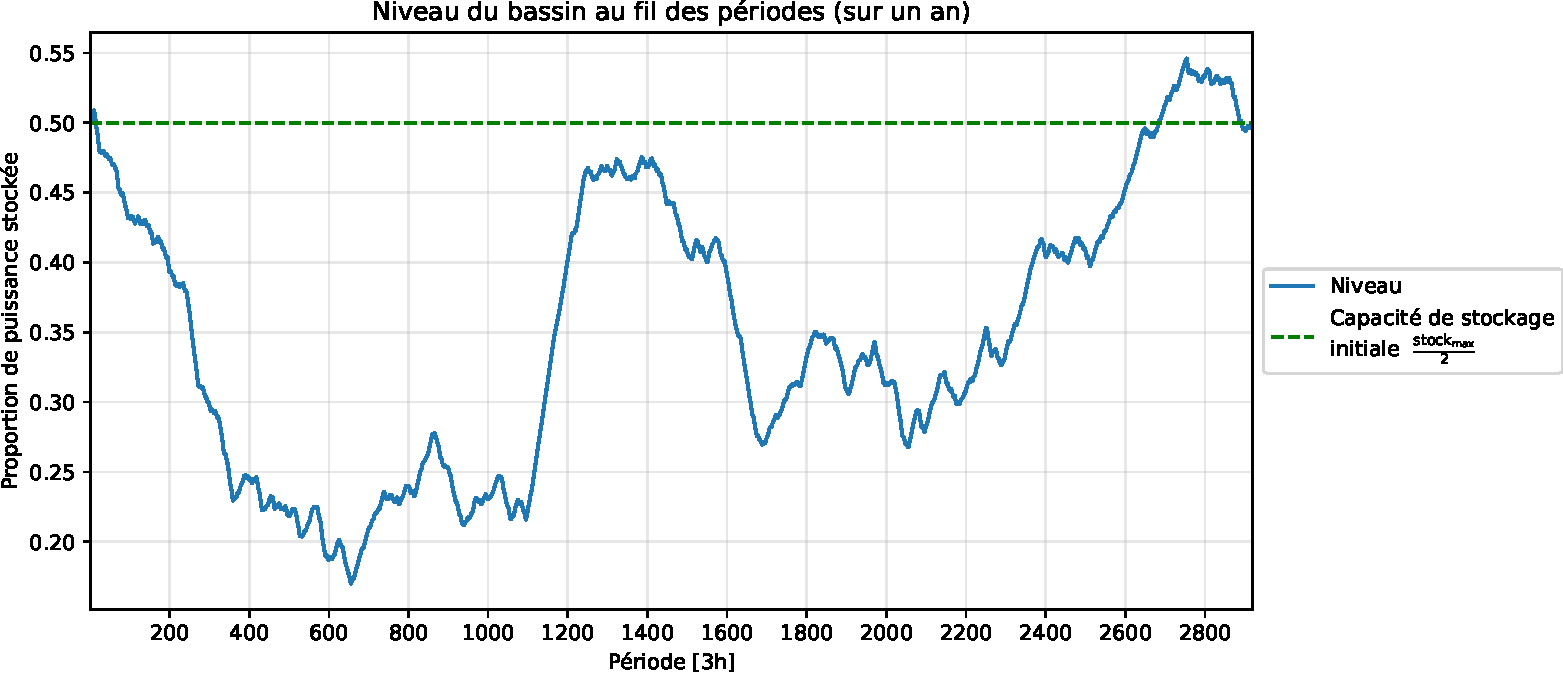
\includegraphics[scale=0.5]{GraphesP2/Niveau_Bassin_Q6.pdf}
    \caption{Représentation graphique du niveau du bassin \eqref{eq:6_contr2} pour le modèle 
    de la question 6 par période de T = 3 heures sur 1000 périodes.} 
    \label{fig:Q62}
\end{figure}

\begin{figure}[H]
    \centering
    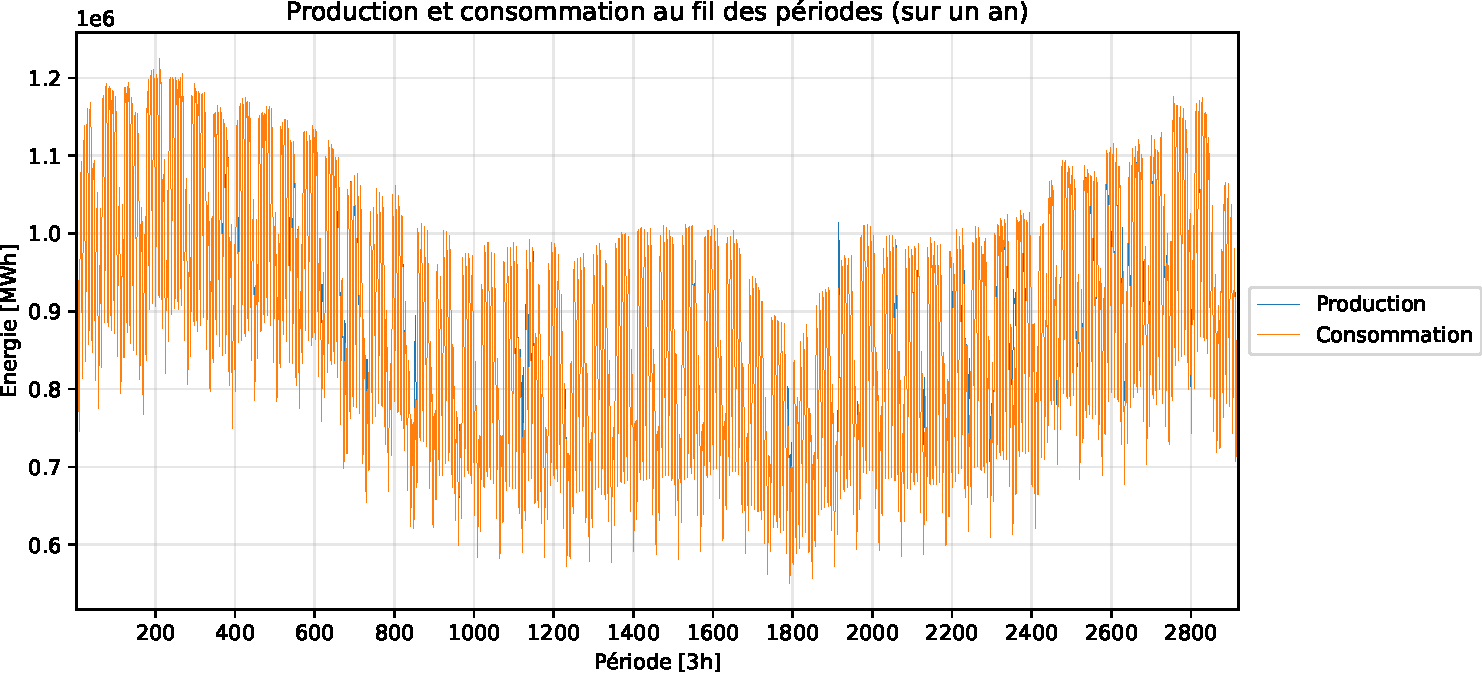
\includegraphics[scale=0.6]{GraphesP2/Prod_Cons_Q6.pdf}
    \caption{Représentation graphique de la production et de la consommation (en MWh) 
    \eqref{eq:6_contr1} pour le modèle de la question 6 par période de T = 3 heures sur un an.} 
    \label{fig:Q63}
\end{figure}
Bien que délicat à bien illustrer, nous pouvons voir que les valeurs de production et de consommation sont 
assez proches.
\end{document}
